Dans le cadre de l'étape de conception, un diagramme de classes représentant le modèle du jeu a été réalisé.

\begin{figure}[!h]
\centering
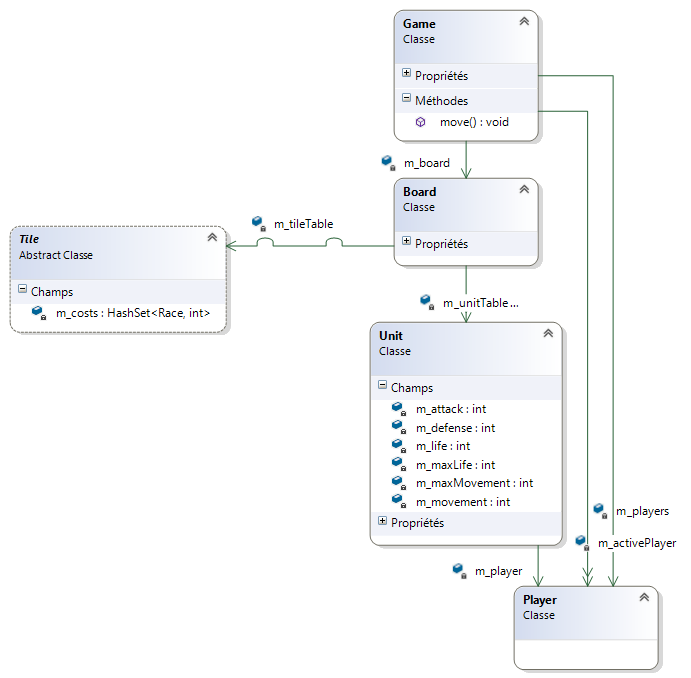
\includegraphics[width=\textwidth]{Parties/Images/UML_Princ.png}
\caption{Les classes princpales de la représentation du jeu}
\label{fig:uml_princ}
\end{figure}

Chaque joueur est représenté par une instance de la classe \emph{Player}.
La classe \emph{Board} contiendra le terrain (sous forme d'instances de \emph{Tile}), ainsi que les unités (instances de \emph{Unit}).
La classe \emph{Game} contiendra le plateau, et sera capable d'appliquer les règles du jeu.